\chapter{Exploratory Data Analysis}
\label{appn:exploration}

\section{Storm Duration}
\label{appn:storm-duration}

\begin{figure}[ht]
    \centering
    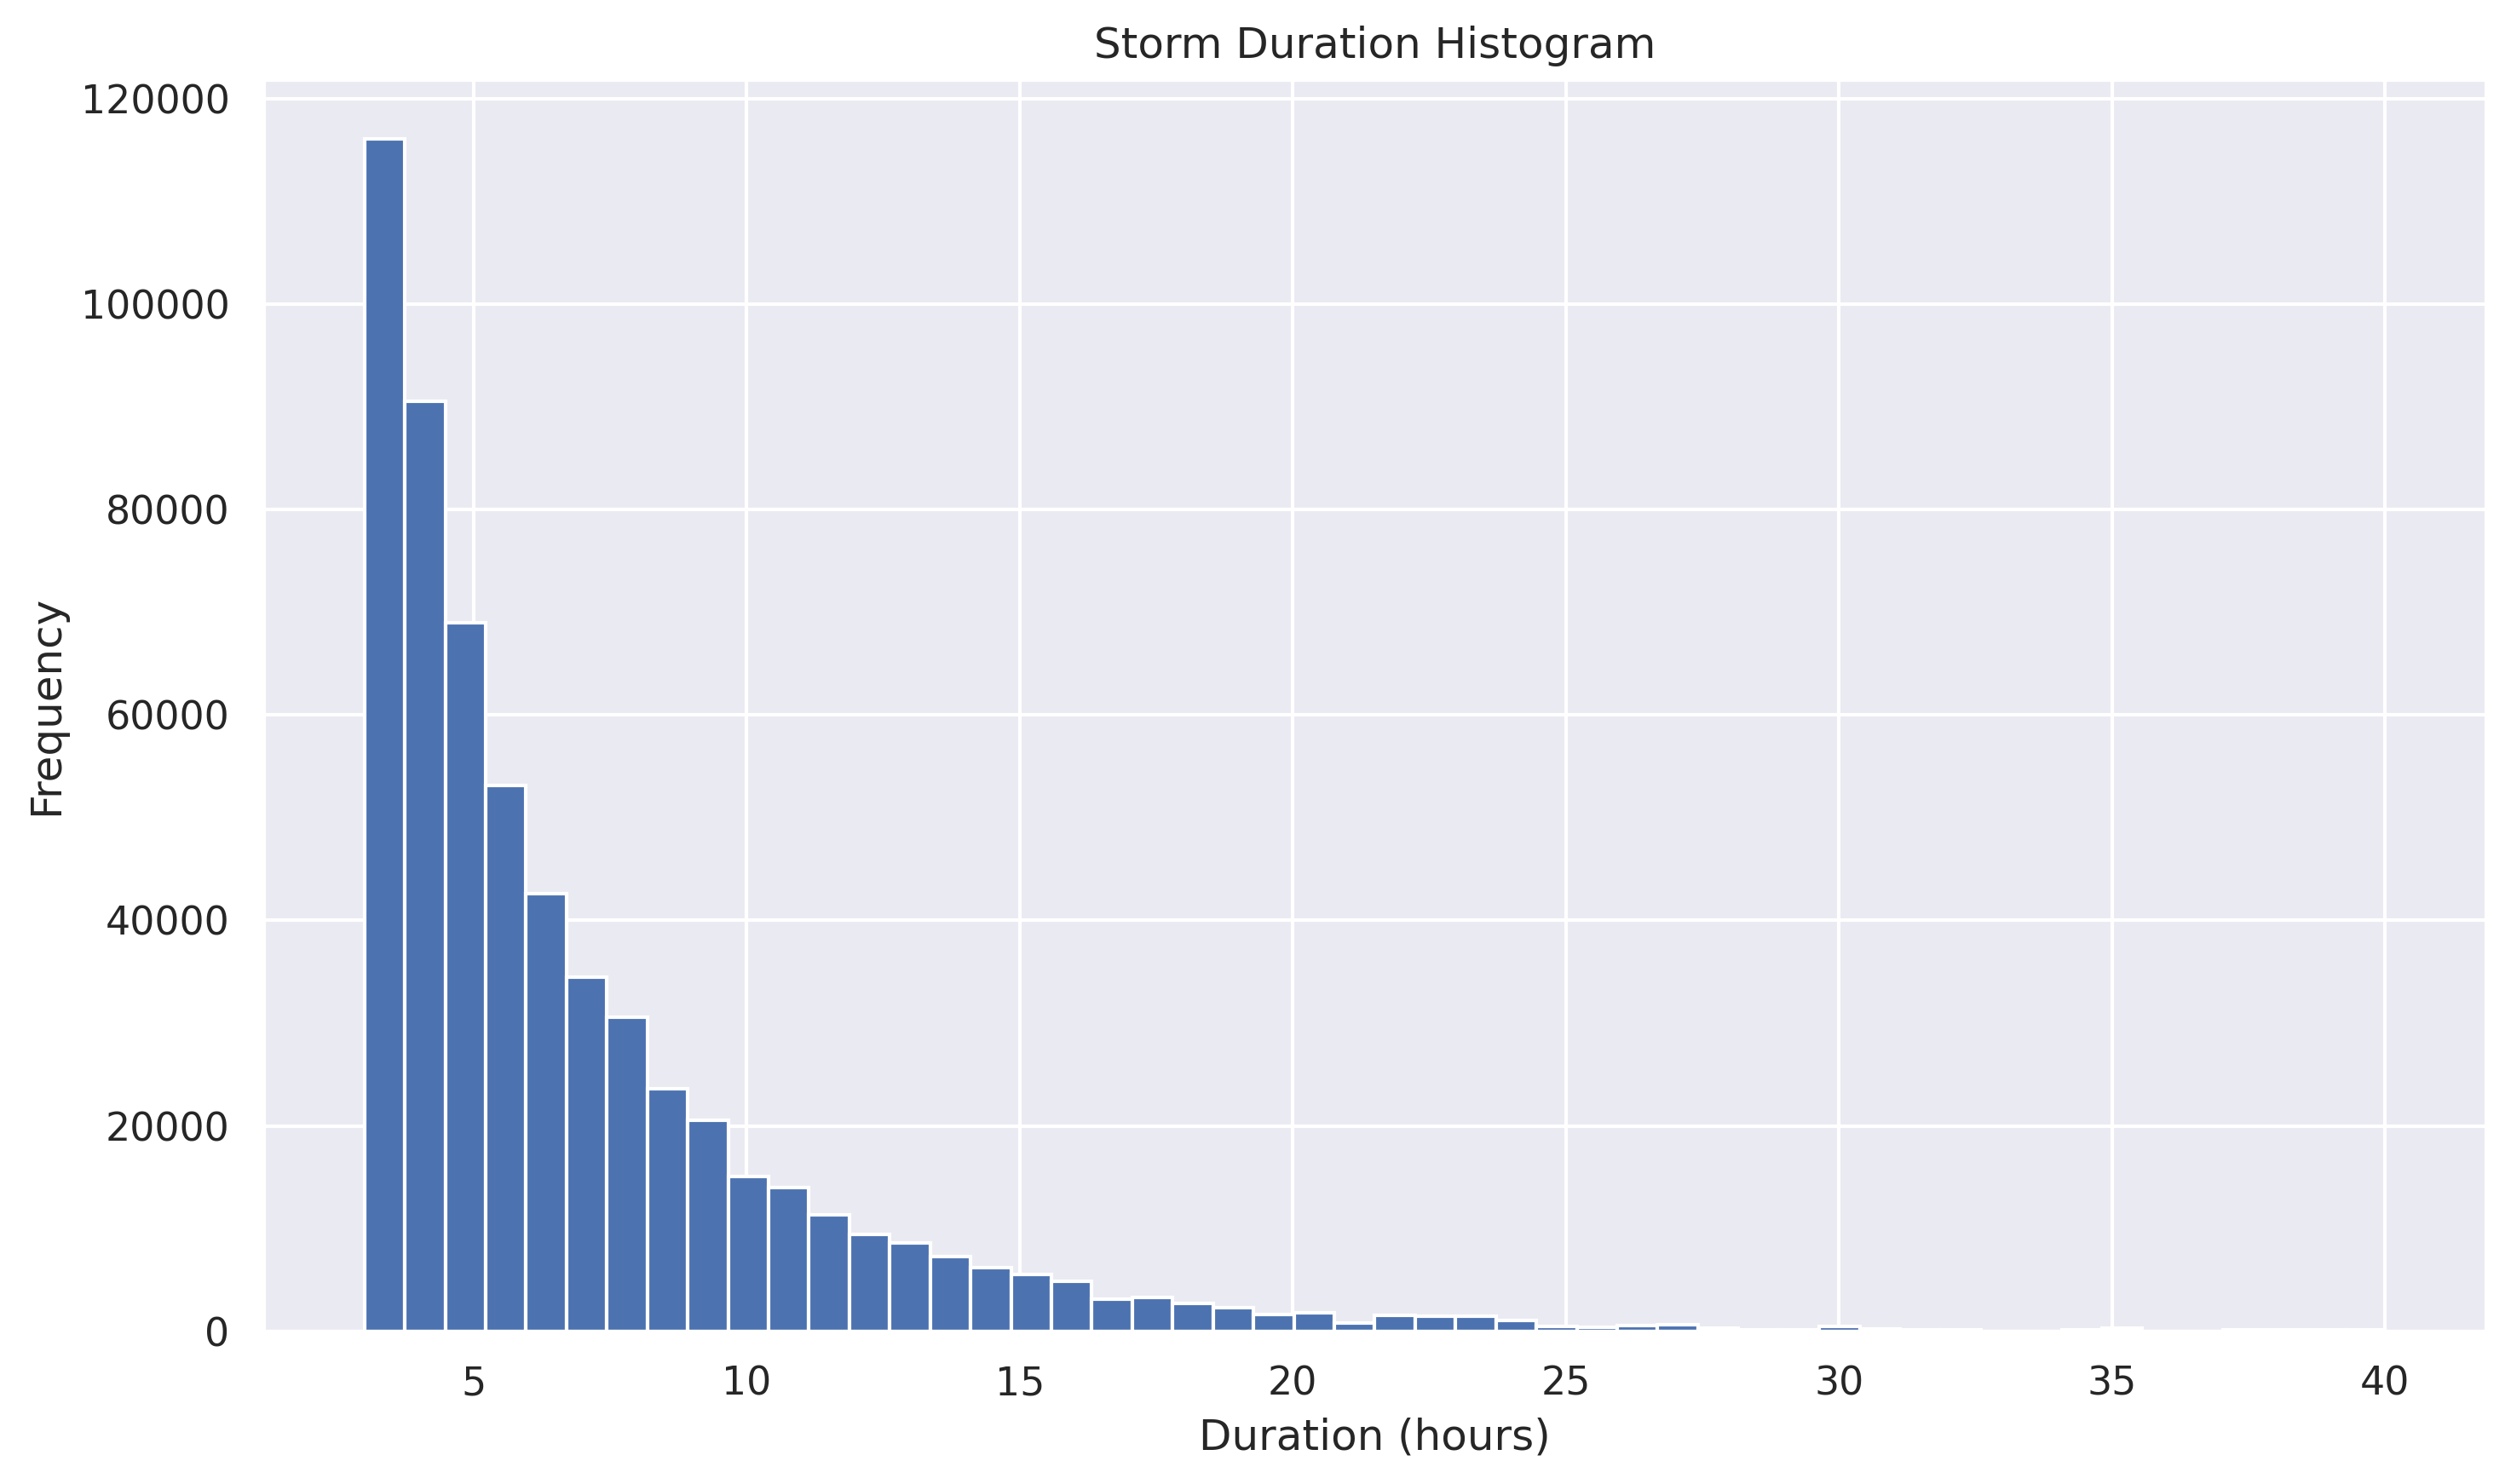
\includegraphics[width=0.8\textwidth]{../figures/generated/exploration/storm_duration_hist.png}
    \caption{Distribution of the storm duration in hours, showing a right-skewed distribution with mean and 95th percentile marked with dashed vertical lines.}
    \label{fig:avg_storm_duration}
\end{figure}

\clearpage

\section{Storm Area}
\label{appn:storm-area}

\begin{figure}[ht]
    \centering
    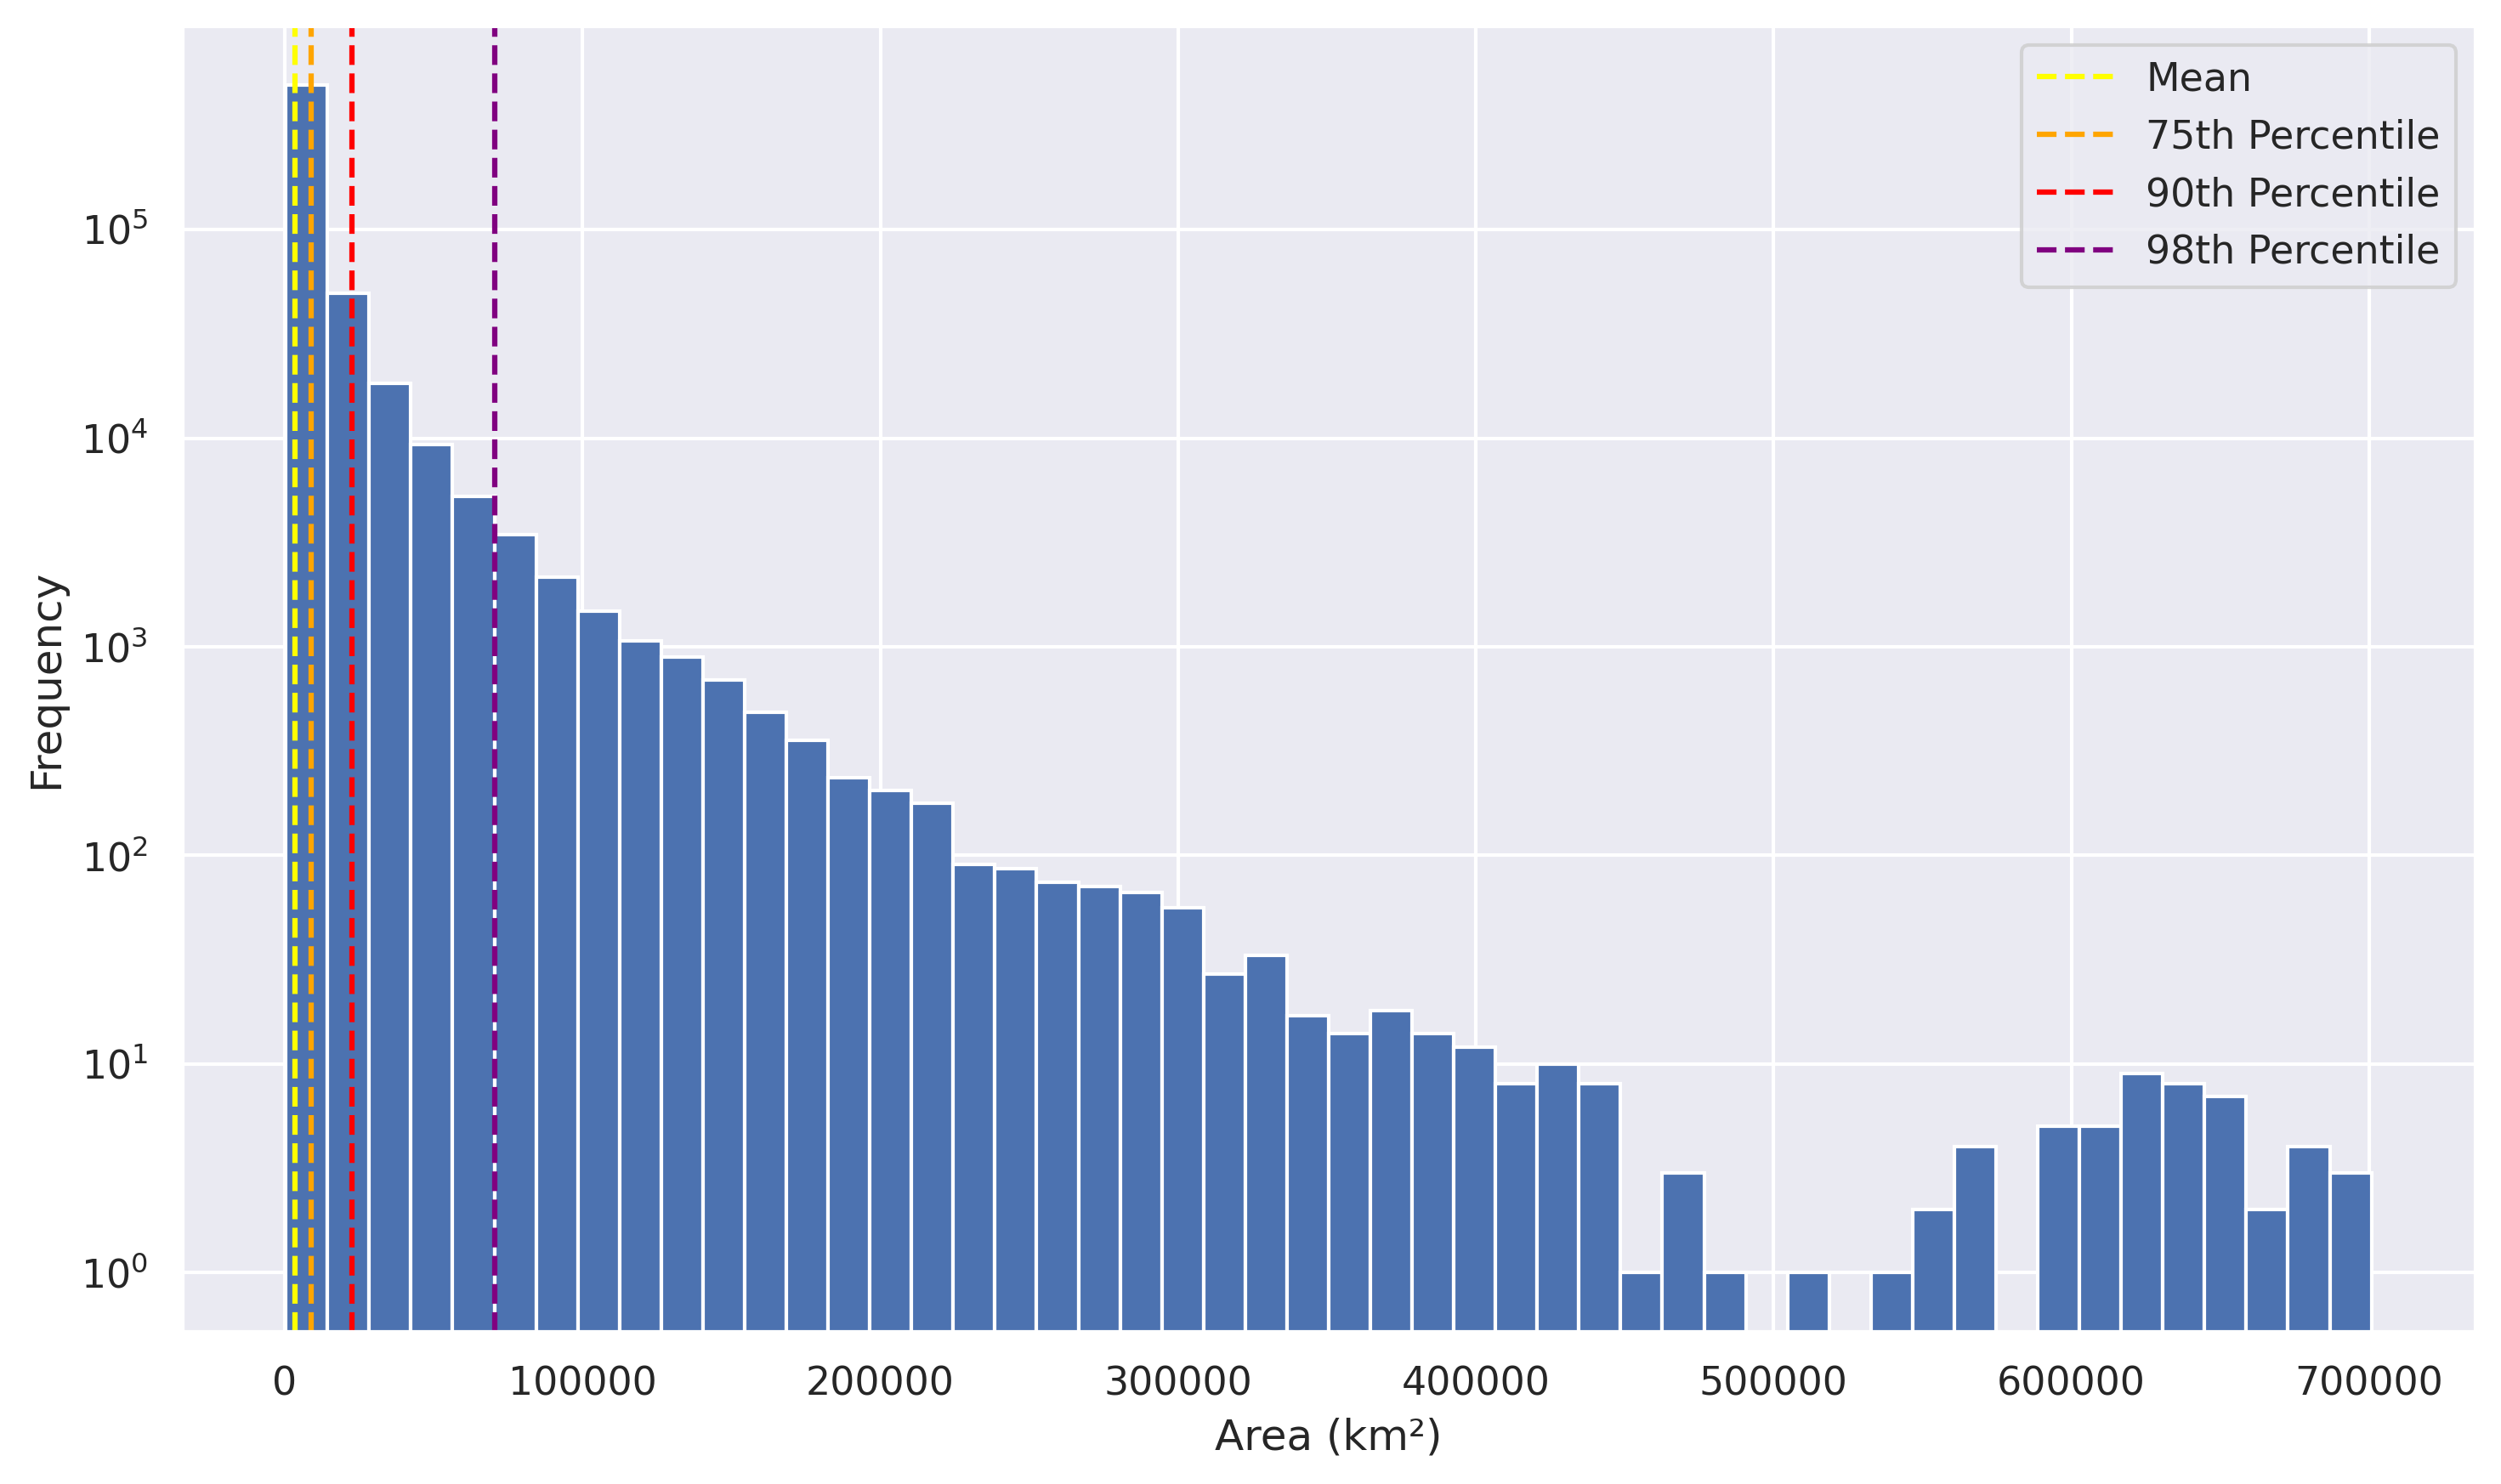
\includegraphics[width=0.8\textwidth]{../figures/generated/exploration/storm_area_hist.png}
    \caption{Distribution of the storm area in square kilometers, showing a right-skewed distribution with mean, 75th, 90th and 98th percentiles marked with dashed vertical lines.}
    \label{fig:avg_storm_area}
\end{figure}
